\documentclass{article}
\usepackage[utf8]{inputenc}

\title{Deep Sparse Rectifier Neural Networks}
\author{}
\date{}

\usepackage{natbib}
\usepackage{graphicx}
\usepackage{amsmath}
\usepackage[left=2.5cm,right=2.5cm,top=1cm,bottom=1.25cm]{geometry}
\usepackage{hyperref}
\usepackage{float}
\usepackage[export]{adjustbox}
\usepackage{sidecap}
\hypersetup{colorlinks=true,urlcolor=blue}
\pagenumbering{gobble}

\begin{document}

\maketitle

\section*{Link}
\href{http://proceedings.mlr.press/v15/glorot11a/glorot11a.pdf}{pdf} 

\section*{Summary}
\begin{itemize}
    \item Studies on brain energy expense suggest that neurons encode information in a sparse and distributed way, estimating the percentage of neurons active at the same time to be between 1 and 4\%. From a computational point of view, such sparse representations are appealing for the following reasons:  
    \begin{itemize}
        \item One of the claimed objectives of deep learning algorithms is to disentangle the factors explaining the variations in the data. A dense representation is highly entangled because almost any change in the input modifies most of the entries in the representation vector. Instead, if a representation is both sparse and robust to small input changes, the set of non-zero features is almost always roughly conserved by small changes of the input.
        \item Different inputs may contain different amounts of information and would be more conveniently represented using a variable-size data-structure. Varying the number of active neurons allows a model to control the effective dimensionality of the representation for a given input and the required precision.
        \item Sparse representations are  more likely to be linearly separable, or more easily separable with less non-linear machinery.
        \item Dense distributed representations are the richest representations, being potentially exponentially more efficient than purely local ones. Sparse(and dense) representations’ efficiency is still exponentially greater, with the power of the exponent being the number of non-zero features.
    \end{itemize}
    However forcing too much sparsity may hurt predictive performance for an equal number of neurons, because it reduces the effective capacity of the model.
    \item Advantages of using ReLU
    \begin{itemize}
        \item The rectifier activation function allows a network to easily obtain sparse representations. For example, after uniform initialization of the weights, around 50\% of hidden units continuous output values are real zeros, and this fraction can easily increase with sparsity-inducing regularization(Figure 1: left). 
        \begin{figure}
            \centering
            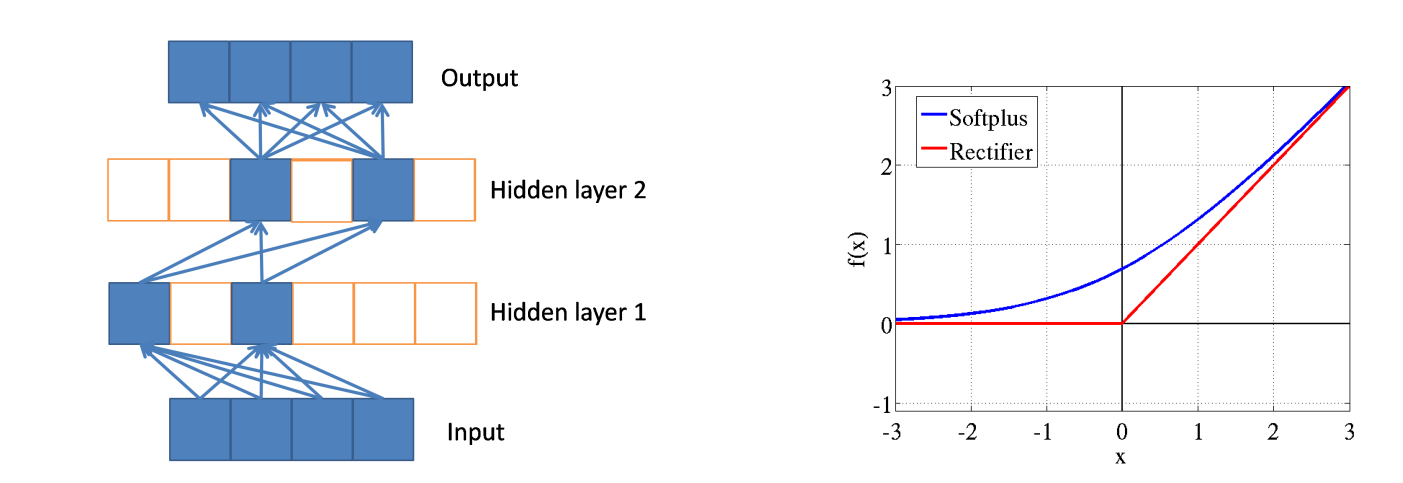
\includegraphics[scale=0.4]{relu.png}
            \caption{Left: Sparse propagation of activations and gradients in a network of rectifier units. Right: Rectifier and softplus activation functions.}
            \label{fig:Figure 1}
        \end{figure}
        \item The function computed by each neuron or by the network output in terms of the network input is linear by parts. Because of this linearity, gradients flow well on the active paths of neurons (there is no gradient vanishing effect due to activation non-linearities of sigmoid or tanh units), and mathematical investigation is easier.
        \item Computations are also cheaper: there is no need for computing the exponential function in activations.
    \end{itemize}
    \item However it may have some disadvantages
    \begin{itemize}
        \item One may hypothesize that the hard saturation at 0 may hurt optimization by blocking gradient back-propagation. To evaluate the potential impact of this effect we also investigate the softplus activation: $softplus(x) = log(1+e^x)$((Figure 1: Right). We lose the exact sparsity, but may hope to gain easier training. However, experimental results tend to contradict that hypothesis, suggesting that hard zeros can actually help supervised training. We hypothesize that the hard non-linearities do not hurt so long as the gradient can propagate along some paths, i.e., that some of the hidden units in each layer are non-zero. With the credit and blame assigned to these ON units rather than distributed more evenly, we hypothesize that optimization is easier.
        \item Another problem could arise due to the unbounded behavior of the activations; one may thus want to use a regularizer to prevent potential numerical problems. Therefore, we use the $L_1$ penalty on the activation values, which also promotes additional sparsity.
        \item In order to efficiently represent symmetric/anti-symmetric behavior in the data, a rectifier network would need twice as many hidden units as a network of symmetric/anti-symmetric activation functions(like $tanh$).
    \end{itemize}
    \item Some of the important experimental observations when using RelU
    \begin{itemize}
        \item Despite the hard threshold at 0, networks trained with the rectifier activation function can find local minima of greater or equal quality than those obtained with its smooth counterpart, the softplus.
        \item There is almost no improvement when using unsupervised pre-training with rectifier activations, contrary to what is experienced using tanh or softplus. 
        \item Rectifier networks are truly deep sparse networks. There is an average exact sparsity (fraction of zeros) of the hidden layers of 83:4\% on MNIST, 72:0\% on CIFAR10, 68:0\% on NISTP and 73:8\% on NORB.
    \end{itemize}
    \item With labeled data, deep rectifier networks appear to be attractive models. They are biologically credible, and, compared to their standard counterparts, do not seem to depend as much on unsupervised pre-training, while ultimately yielding sparse representations.
\end{itemize}

\end{document}
